\documentclass[journal,twoside]{IEEEtran}

\usepackage{texnames}
\usepackage{graphicx}
\graphicspath{{../Figures/PDF/}{../Figures/PNG/}}
\DeclareGraphicsExtensions{.pdf,.png,.jpg,.jpeg}

\usepackage{color}
\usepackage{amsmath}
\interdisplaylinepenalty=2500
\usepackage{algorithmic}
\usepackage{array}
\usepackage[font=footnotesize,margin=1ex]{subcaption}
%\usepackage{dblfloatfix}
%\usepackage[nomarkers]{endfloat}
\usepackage{url}
\usepackage{booktabs}

%\usepackage{tikz}
%\usetikzlibrary{shapes.geometric,arrows,trees}
%
%
%\tikzstyle{root} = [rectangle, rounded corners, minimum width=2cm, minimum height=.7cm, text centered, draw=black, fill=blue!30]
%\tikzstyle{files} = [rectangle, minimum width=1cm, minimum height=.5cm, text centered, draw=black, fill=white]
%\tikzstyle{link} = [thick, -]

\begin{document}
	
\title{Proposal of a Badging System for Reproducibility in Remote Sensing Research}
	
\author{Alejandro~C.~Frery,~\IEEEmembership{Senior Member,~IEEE,}
Luis~Gomez,~\IEEEmembership{Senior Member,~IEEE,}
and~Qi~Wang,~\IEEEmembership{Senior Member,~IEEE}% <-this % stops a space
\thanks{A.\ C.\ Frery is with the \textit{Laborat\'orio de Computa\c c\~ao Cient\'ifica e An\'alise Num\'erica} -- LaCCAN, Universidade Federal de Alagoas, Macei\'o, Brazil, and with the Key Lab of Intelligent Perception and Image Understanding of the Ministry of Education, Xidian University, Xi'an, China. (email: acfrery@laccan.ufal.br)}% <-this % stops a space
\thanks{Luis Gomez is with the Universidad de Las Palmas de Gran Canaria, Spain}% <-this % stops a space
\thanks{Qi Wang is with the Northwestern Polytechnical University, China}% <-this % stops a space
\thanks{Manuscript received XX, accepted YY.}}
	
\markboth{IEEE Journal of Selected Topics on Applied Earth Observations and Remote Sensing,~Vol.~XX, No.~YY, Month~2020}%
{Frery \MakeLowercase{\textit{et al.}}: Badging Reproducibility and Replicability}
	
\maketitle
	
\begin{abstract}
\textcolor{red}{Remote Sensing is a truly active research area, where many actors play a fundamental role, from industry (public or private) to large or small research groups. 
From that intensive activity, methods, algorithms and techniques are continuously published or broadcasted through papers, conferences, repositories or other means. 
In most cases, there is a sound interest from researchers to use those methods, what implies easy availability of the related methods (computational codes or more detailed descriptions) and implicitly, that method have been extensively tested and they are ready for its use. 
Reproducibility research comprises all those issues just mentioned. In this paper, we aim to provide insights to complement the visibility of research in the area of Remote Sensing and, what is considered more relevant: to \textit{seduce} Authors to include those resources  in their common scientific activity.}
\end{abstract}
	
\begin{IEEEkeywords}
Reproducibility,
Replicability,
Remote Sensing
\end{IEEEkeywords}
	

\IEEEpeerreviewmaketitle

\section{Rationale}\label{Sec:Introduction}

\IEEEPARstart{R}{eproducibility} is at the core of experimental sciences. 
It is also a basilar element of scientific integrity. 
The advent of data science is leading to new requirements and practices able to cope with the challenges posed by huge volumes of data, often of dynamic nature. 

Modern grounds for Reproducible Research were set before the widespread use of deep learning and other massively data-based techniques. 

Among the efforts made towards building Remote Sensing Reproducible Research environments, one may mention Code Ocean and GRSS Remote Sensing Code Library. 
These two initiatives belong to the IEEE scientific ecosystem. 

However, is this enough for healthy science in Remote Sensing? 
We do not think so. 
Many authors continuously strive to disseminate their research findings in such a way that any user will be able to validate them at a later stage. 
This includes the proposal of software architectures, the use of open data, FLOSS (Free/Libre Open Source Software), and other initiatives.

Barba~\cite{TerminologiesforReproducibleResearch} identifies several usages of the terms ``Reproducibility'' and ``Replicability,'' and also the emergence of the term ``Repeatability,'' among others.

We will discuss two core concepts: Reproducibility and Replicability, in order to simplify the discussion and to arrive to the suggestion of good scientific practices.

We will use the metaphor of dwarfs standing on the shoulders of giants which, in the words of Isaac Newton~\cite{LetterNewton}, is
\begin{quote}
	If I have seen further it is by standing on the shoulders of Giants.
\end{quote}
Reproducibility consists in allowing the whole community reach your shoulders.
Replicability grants the community to stand on your shoulders.

A scientific work is reproducible if other researchers can obtain the data and the code and, effortlessly, obtain the same products (analyses and reports).
A scientific work is replicable if it reported in such a way that other researchers can perform similar studies and arrive to compatible conclusions.

Quoting Ref.~\cite{PraxisofReproducibleComputationalScience}:
\begin{quote}
	a promise in a published paper
	to make code and/or data ``available upon
	request'' is not a reproducible practice: digital
	artifacts should already be in a suitable repository.
\end{quote}


\section{Badging Systems}

Are striving to recognize those articles that comply with reproducibility criteria by assigning badges.
In the sequel, we mention two of those initiatives.

To date, sixty seven journals use the Open Science badging system\footnote{https://cos.io/our-services/open-science-badges/}.
It consists of three levels: (a)~Open Data, (b)~Open Materials, and (c)~Preregistered study; cf.\
Fig.~\ref{Fig:OpenScienceBadges}
According to Munaf\`o et al.~\cite{ManifestoReproducibleScience}, this practice increased by an order of magnitude articles with open data in the \textit{Psychological Science} journal.

\begin{figure}[hbt]
	\centering
	\subcaptionbox{Open Data}{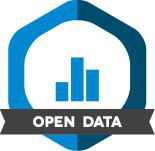
\includegraphics[width=.2\columnwidth]{OpenData}}
	\subcaptionbox{Open Materials}{
\includegraphics[width=.2\columnwidth]{OpenMaterials}}
	\subcaptionbox{Preregistered}{
\includegraphics[width=.2\columnwidth]{Preregistered}}
	\caption{Open Science three-level badging system}\label{Fig:OpenScienceBadges}
\end{figure}

ACM -- The Association for Computing Machinery has a five-level badging system\footnote{ \url{https://www.acm.org/publications/policies/artifact-review-badging}}, illustrated in Fig.~\ref{fig:ACM-Badging}.

\begin{figure}[hbt]
	\centering
	\subcaptionbox{Functional artifacts\label{Fig:Functional}}{
\includegraphics[width=.19\columnwidth]{artifacts_evaluated_functional}}
	\subcaptionbox{Reusable artifacts\label{Fig:Reusable}}{
\includegraphics[width=.19\columnwidth]{artifacts_evaluated_reusable}}
	\subcaptionbox{Available artifacts\label{Fig:Available}}{
\includegraphics[width=.19\columnwidth]{artifacts_available}}
	\subcaptionbox{Reproducible results\label{Fig:Reproducible}}{
\includegraphics[width=.19\columnwidth]{results_reproduced}}
	\subcaptionbox{Replicable results\label{Fig:Replicable}}{
\includegraphics[width=.19\columnwidth]{results_replicated}}
	\caption{ACM five-level badging system}\label{fig:ACM-Badging}
\end{figure}

It is worth noting that levels~\ref{Fig:Functional} and~\ref{Fig:Reusable} do not grant \textit{per se} reproducibility.
They just acknowledge that the authors made their code available to reviewers, and that it is functional and reusable.
The remote sensing community should strive to attain, at least, level~\ref{Fig:Reproducible}.

We believe that a similar, even if simpler, badging system will have great positive impact in the remote sensing community.

\section{IEEE Platforms}

\subsection{Code Ocean}

\subsection{GRSS Code Library}

\section{Proposal}

\subsection{Requirements}

\subsubsection{Web page}\label{Sec:WebPage}
The first requisite for being considered a RSRR is associating the manuscript to a universally accessible and informative web page containing:
\begin{enumerate}
	\item\label{item:ProjectID} Project identification (one project may host more than one paper; one paper may be hosted by more than one project)
	\begin{enumerate}
		\item Title
		\item Participants
		\item Summary
		\item Funding information
		\item Start date, state (in preparation, active, finished)
	\end{enumerate}
	\item Paper identification (if different from~\ref{item:ProjectID})
	\begin{enumerate}
		\item Title
		\item Contact: the corresponding author
		\item Abstract
		\item PDFs of relevant versions, including information of its submission to repositories (arXiv, etc.), journal or conference
		\item\label{item:SourceDocumentFiles} \LaTeX\ and \BibTeX\ files, images, and plots
	\end{enumerate}
	\item\label{item:Platform} Computational platform (machine, model, operating system, software, libraries, and versions)
	\item Code (with comments)
	\item Data
	\item Which software components are FLOSS or free (including operating system)?
	\item Provide precise instructions and examples about:
	\begin{enumerate}
		\item How to install and run the code;
		\item How to read and modify the data;
		\item How to generate the plots, images (where they improved for visualization? how?), and tables (rounding, truncating, etc.)
	\end{enumerate}
\end{enumerate}

\subsubsection{Experimental design} Many studies rely on the information provided by samples;
few of them detail the procedure with which they were collected.
A reproducible study should, besides providing the samples used, state the following:
\begin{enumerate}
	\item Objective criteria set \textit{a priori} for sample collection.
	\item Number of samples, sample size, and descriptive statistics for the aggregated data.
	\item Objective criteria for sample selection and data imputation.
\end{enumerate}

Stochastic simulation is at the core of randomized algorithms as, for instance, Monte Carlo experiments.
In order to make such algorithms reproducible, apart from the information in Section~\ref{Sec:WebPage}, item~\ref{item:Platform}, the authors must inform the pseudo-random number generator and the seeds employed.

Science is not only made of positive results.
Sticking to this path may restrict the outcomes to confirmatory studies, avoiding those lines of research that do not produce immediately publishable results.
Scientific honesty requires telling the whole story, starting from clearly defining the research protocol~\cite{TellItlikeItIs}.
The research course may change along the work, but telling the whole story adds more to the scientific knowledge that reporting only the evidence and the conclusions that are aligned with the starting hypotheses.


\subsubsection{Open data}

\subsubsection{Free/Libre Open Source Software}

\subsubsection{Code}

\subsubsection{Text}

\subsection{Implementation}

GRSS should implement a Remote Sensing Reproducibility Committee for each of its (currently) four journals, namely:
IEEE Transactions on Geoscience and Remote Sensing,
IEEE Geoscience and Remote Sensing Letters,
IEEE Geoscience and Remote Sensing Magazine, and
IEEE Journal of Selected Topics on Applied Earth Observations and Remote Sensing.
This committee will act solely on accepted papers for which the authors have requested the RSRR Badge.

The the assessment process has three possible outcomes:
\begin{description}
	\item[Fully RSRR:]
	\item[Partially RSRR:] 
	\item[No badge:]
\end{description}

Some of the direct benefits for papers published under the RSRR Badge are
\begin{itemize}
	\item the paper will display the recognition (both for the paper printed and for the online versions),
	\item the paper will be specially promoted after publication by the Journals,
	\item the journal will enforce, in each cross-referenced database, that the paper has that badge recognition.
\end{itemize}

As authors' obligation, a pre-requisite to obtain the badge is the acknowledgement that the paper is Reproducible in all the terms for a period of at least five years.

\section{Tools}

Starting well saves lots of time.
We make recommendations that may save time and efforts.
All of them are either free, or offer a free operational version which usually suits the needs of relatively small remote sensing reproducible research projects.

\subsection{Doodling}

Doodling is an important stage to unlock creativity in a controlled manner.
We suggest using FreeMind\footnote{\url{http://freemind.sourceforge.net/wiki/index.php/Main_Page}}, or any other mind map tool, for this purpose.

Figure~\ref{Fig:Doodle} shows the mind map product of such doodling stage.
It served as guide for the structure of this paper.

\begin{figure}[hbt]
\centering
\includegraphics[width=\linewidth]{"Badging RSRR.pdf"}
\caption{The mind map that led to this paper}\label{Fig:Doodle}
%%% The source is in /Figures/FreeMind/Badging RSRR.mm
\end{figure}

Having such an editable visual structure, along with properties and relationships between elements, helps reminding and documenting the progress of the project.

\subsection{Git repository}

We assume in this section that you use \LaTeX\ and \BibTeX.

The main idea consists in having a single repository for all the scientific texts you write: 
theses, 
reports, 
articles, 
letters,
reviews,
and miscellaneous documents.

Fig.~\ref{Fig:StructRepo} illustrates the recommended basic structure for a repository holding several \LaTeX\ files (or projects), along with their associated data and code.

\begin{figure}[hbt]
	\centering
	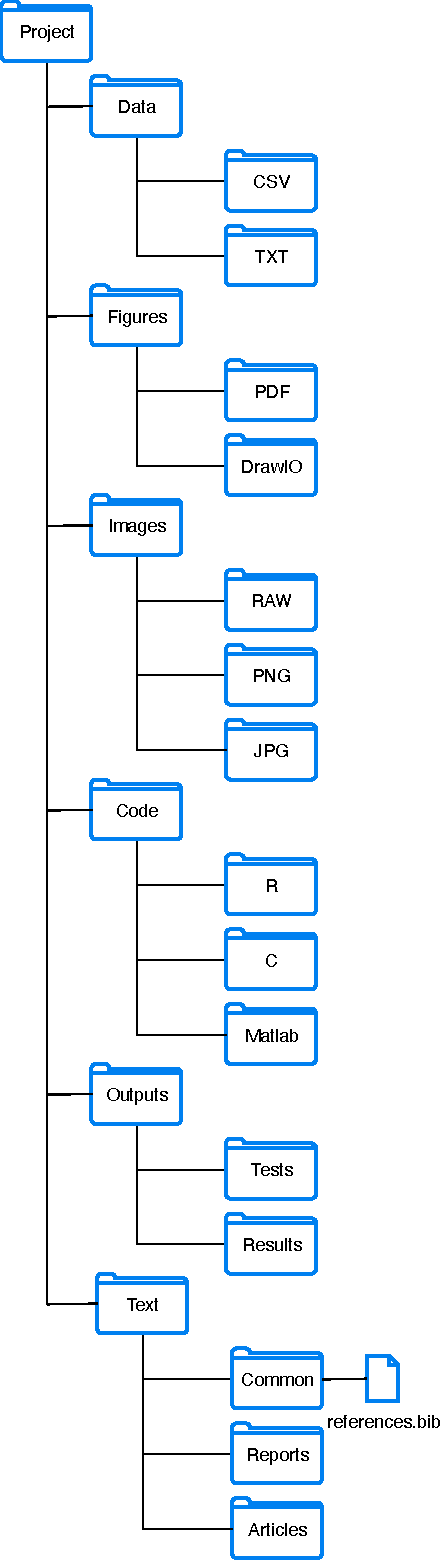
\includegraphics[width=.35\columnwidth]{DirectoryStructure}
	\caption{Recommended structure of a repository for scientific projects.}\label{Fig:StructRepo}
	%%% The source is in /Figures/DrawIO/DirectoryStructure.drawio
\end{figure}

Every directory may contain specific subdirectories.
For instance, \verb|Data| may contain \verb|CSV|, \verb|text|, and other directories with specific data files.

Notice that there is a single \BibTeX\ file (with extension \verb|.bib| in the \verb|Common| directory).
\BibTeX\ references can be split on several files, but these files should be common to all projects.
This avoids outdated and redundant bibliographic data bases.

Every article should be in its own directory.
Avoid using the name of the journal where you will submit your work for the directory and document names, as the destination may change along the process.

Data, figures, images and code should be common to all projects, as one typically reuses them.
Inform in your \LaTeX\ code the source of each figure, for instance with a comment of the form \texttt{\%\%\% The source is in /Figures/DrawIO/DirectoryStructure.drawio}.
This will help the review process, and the communication between authors.

Check Ref.~\cite{EditorialGRSL2015} for a naming convention and suggestions for revision handling of submitted manuscripts.

\subsection{Communication}

Most of the research in remote sensing is collaborative, and involves two or more authors.
This is mostly due to the interdisciplinary nature of the area, which requires complementary competencies.
Communication in such scenario is of paramount importance.

Although e-mail is a powerful tool, synchronous communication is often required.
WhatsApp and WeChat are the commonplace for real-time exchange of ideas, but they do not offer either the tools or the organization required for prolific and time-saving technical conversations.

Slack\footnote{\url{https://slack.com/}} serves this purpose well.
It organizes conversations in channels, connects with other applications (Google Suit, meetings, Github, polls, etc.) promoting, thus, focus and persistence.

\subsection{Task management}

We have stressed the importance of using a Kanban-style management method for building a project~\cite{SuccessfulScientificPublishingfromtheProjecttotheAdvertising}.
Such method is also recommended for simple task management.
Although a more sophisticated tool, such as ProjectLibre\footnote{\url{https://www.projectlibre.com/}} is highly advisable for projects which involve several participants, resources, deliverables, and deadlines, the process of organizing and maintaining a remote sensing reproducible project is usually well met by Trello\footnote{\url{https://trello.com/}}.

Fig.~\ref{Fig:ScientificCanvas} shows the structure of a Scientific Canvas in Trello, freely available at \url{https://trello.com/b/C747M1GX}.
Cards are organized in lists, and lists in groups.
This board can be copied, and assigned to a team, whose leader can assign tasks (cards), with deadlines, reminders, and several other utilities.

\begin{figure}[hbt]
\centering
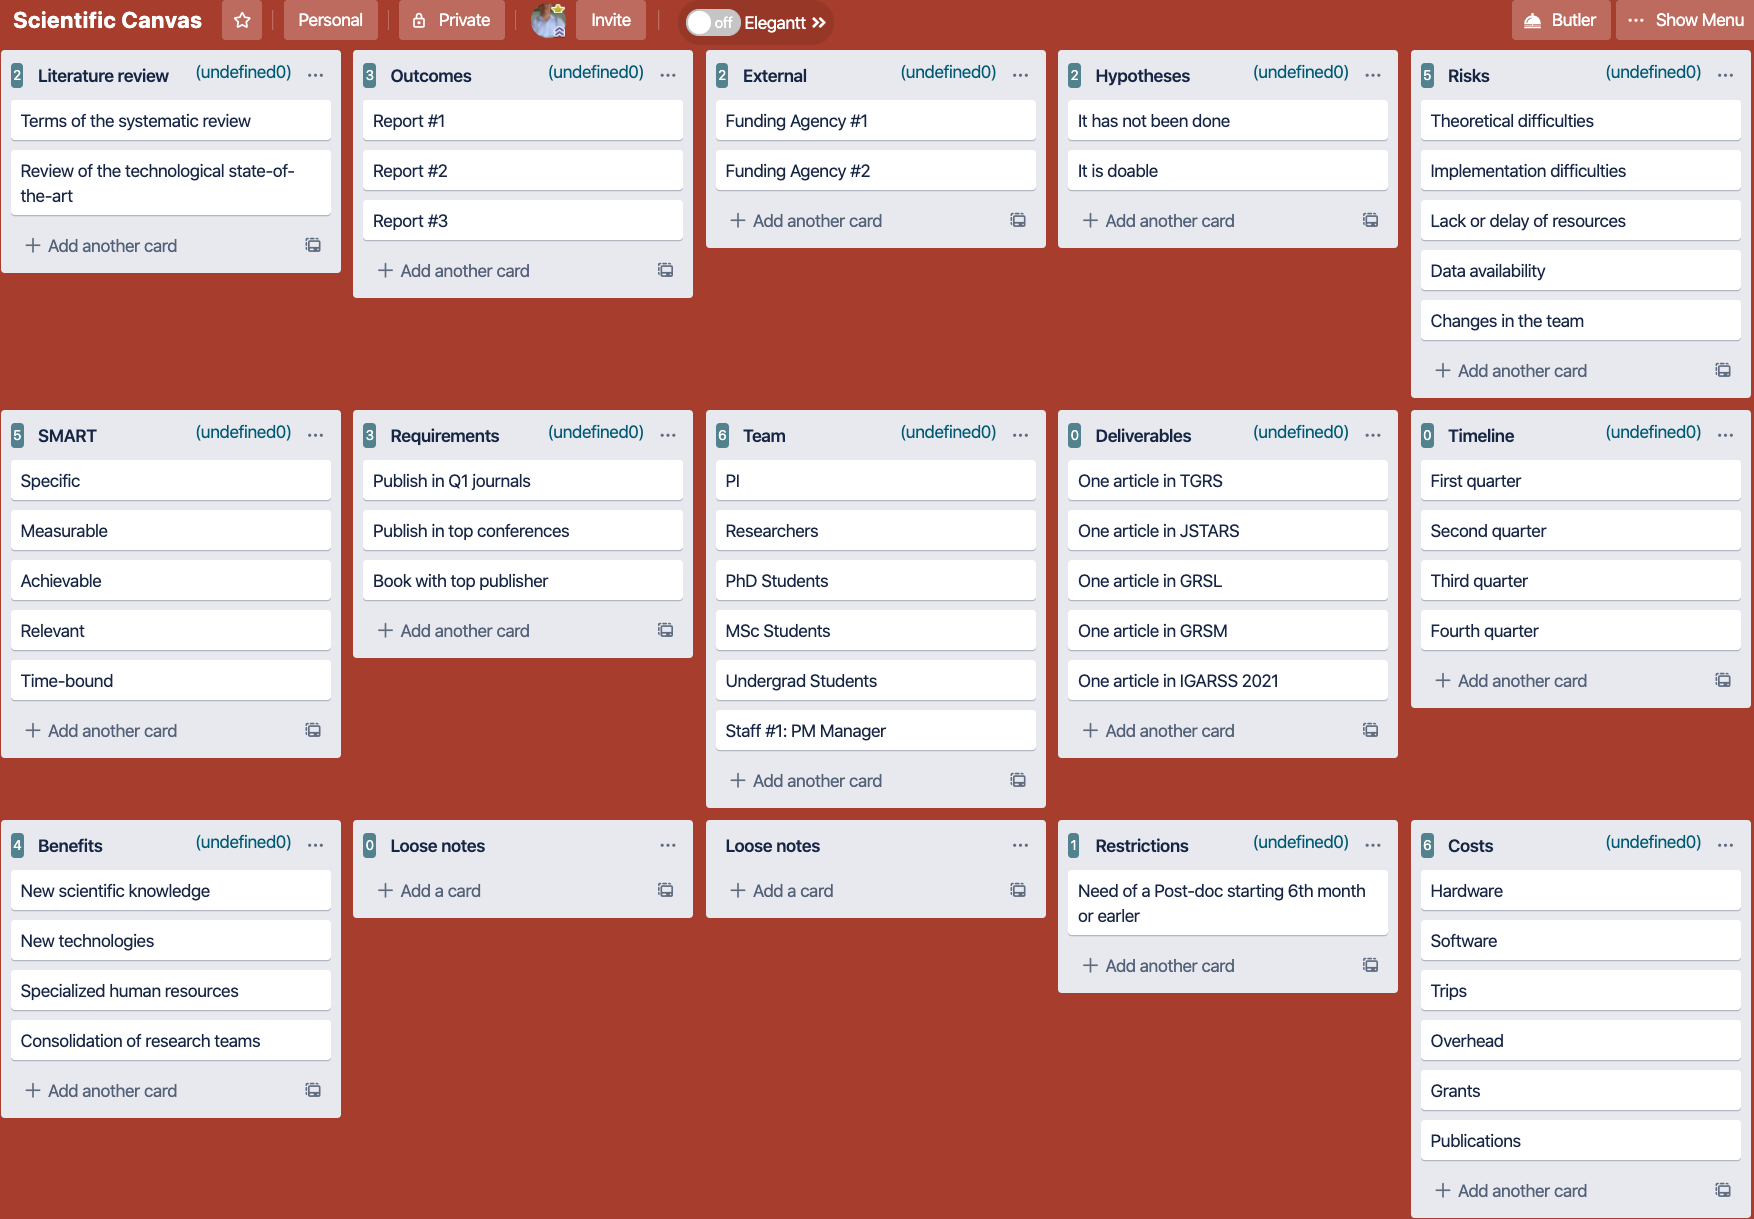
\includegraphics[width=\linewidth]{ScientificCanvas}
\caption{A Trello implementation of a Scientific Canvas}\label{Fig:ScientificCanvas}
\end{figure}

As Trello keeps track of every single modification, it becomes a useful resource when it comes to reproducibility.

\section{Challenges}

	
\section*{Acknowledgments}
The authors would like to thank...
	
\nocite{StatisticalAnalysesReproducibleResearch,%
RRComputationalHarmonicAnalysis,%
RREconometrics,%
RRSignalProcessing,%
AddressingNeedDataCodeSharingComputationalScience,%
ReproducibleResearchinComputationalScience,%
TenRulesReproducibleComputationalResearch,%
AddressingNeedDataCodeSharingComputationalScience,
SevenReasonsWhyaUsersGuidetoTransparencyandReproducibility,%
OutoftheBoxReproducibilityaSurveyofMachineLearningPlatforms,%
ReproducibilityofScientificResults2018,%
ReproducibleResearchandGIScienceanEvaluationUsingAGILEConferencePapers,%
TheStateofReproducibilityintheComputationalGeosciences}
	
\bibliographystyle{IEEEtran}
\bibliography{./Common/references}

	
\end{document}



